% Number 360
% CAPMG 
% Token toss - qual graph stack describing motion, avg v
% JG

% Watermark
\AddToShipoutPicture*{\BackgroundPic}

\addtocounter {ProbNum} {1}

\begin{floatingfigure}[r]{.15\textwidth}
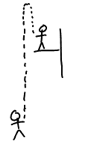
\includegraphics[scale=.8]{/Users/jgates/desktop/latex/pics/tokentoss.png}
\end{floatingfigure}
 
{\bf \Large{\arabic{ProbNum}}} A man, on the ground, throws a subway token to his friend on the platform above.  The token is thrown essentially straight up; it flies past the friend and falls back to him. Call the lower man�s hand ${y=0}$ and define �up� as positive.

\bigskip  Draw graphs of the token�s vertical position, velocity, and acceleration during the trip.  No numbers are necessary.
Make sure that the time scales of the three graphs line up.

\begin{center}
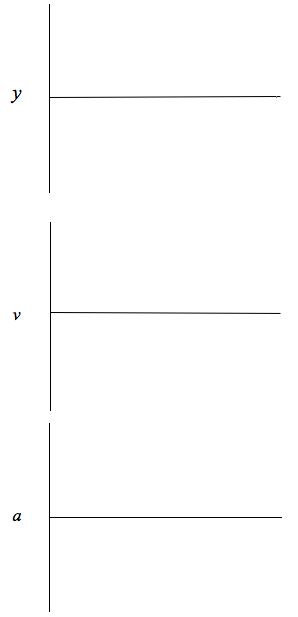
\includegraphics[scale=.85]{/Users/jgates/desktop/latex/pics/blankyvagraphstack.png}
\end{center}

\bigskip Finally, show on both the position and velocity graphs the \emph sign (is it positive, negative, or zero?) of the average velocity for the trip.  Be sure that it�s clear which characteristic of each graph you used to determine the sign of the average velocity!

\vfill
\newpage